\documentclass[tikz, varwidth=600pt]{standalone}
\usepackage[T1]{fontenc}
\usepackage{lmodern}
\usepackage{amssymb, amsmath,bbm}

\standaloneenv{aaaa}

\begin{document}
	\begin{aaaa}
		\begin{center}	
		\fbox{%
			\begin{minipage}{0.85\linewidth}
				\centering
				\tikzset{every picture/.style={line width=0.75pt}} %set default line width to 0.75pt        
				\vspace{6pt} 
		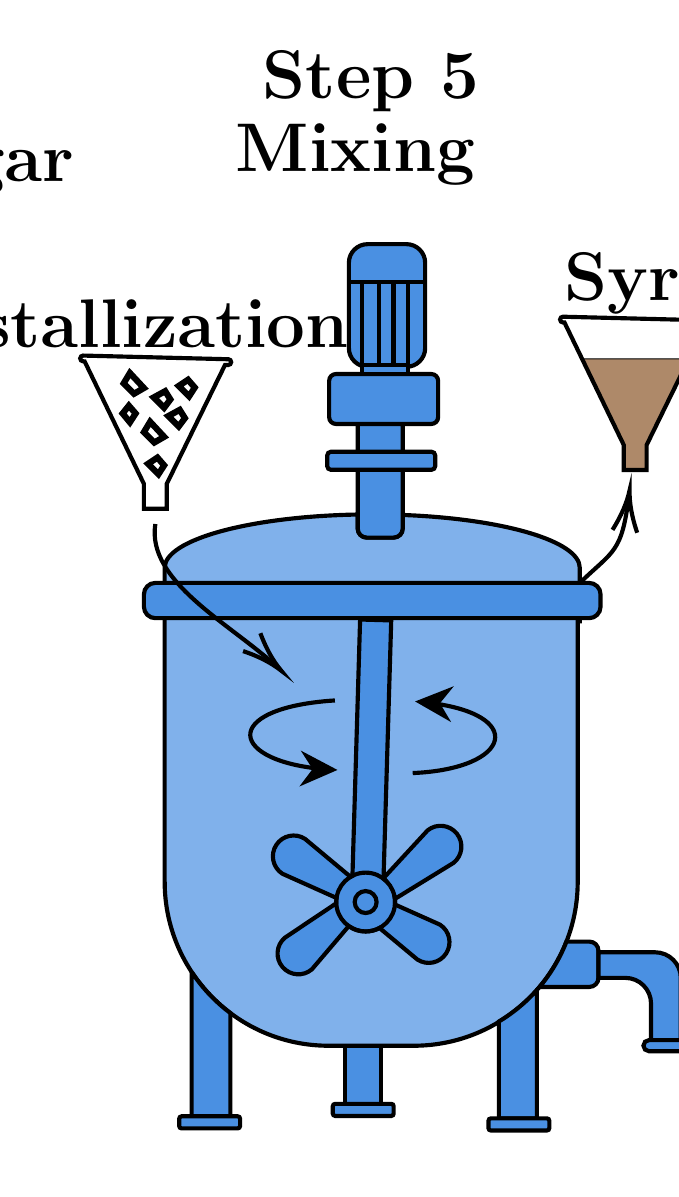
\begin{tikzpicture}[x=0.75pt,y=0.75pt,yscale=-1,xscale=1]
			%uncomment if require: \path (0,552); %set diagram left start at 0, and has height of 552
			    \path[use as bounding box] (400,0) rectangle (700,550);
			\begin{scope}[xshift=183pt]
			%Shape: Path Data [id:dp5133413453165715] 
			\draw  [fill={rgb, 255:red, 74; green, 144; blue, 226 }  ,fill opacity=0.7 ][line width=1.5]  (342,490.5) -- (301,490.5) .. controls (257.37,490.5) and (222,455.13) .. (222,411.5) -- (222,260.25) .. controls (222,246.63) and (263.04,235.49) .. (315,234.56) -- (315,241.33) .. controls (315,243.73) and (316.94,245.67) .. (319.33,245.67) -- (332.33,245.67) .. controls (334.73,245.67) and (336.67,243.73) .. (336.67,241.33) -- (336.67,234.77) .. controls (384.94,236.6) and (422,247.31) .. (422,260.25) -- (422,286) -- (421,286) -- (421,411.5) .. controls (421,455.13) and (385.63,490.5) .. (342,490.5) -- cycle ;
			%Shape: Path Data [id:dp5565946051651287] 
			\draw  [fill={rgb, 255:red, 74; green, 144; blue, 226 }  ,fill opacity=1 ][line width=1.5]  (362.79,388.33) .. controls (366.23,392.66) and (365.5,398.96) .. (361.17,402.4) -- (333.33,419.5) -- (332.71,418.4) .. controls (332.9,419.33) and (333,420.29) .. (333,421.27) .. controls (333,421.67) and (332.98,422.07) .. (332.95,422.46) -- (354.66,432.17) .. controls (359.3,435.18) and (360.62,441.38) .. (357.61,446.03) .. controls (354.6,450.67) and (348.4,451.99) .. (343.76,448.98) -- (325.51,433.77) .. controls (323.52,434.83) and (321.25,435.44) .. (318.83,435.44) .. controls (315.8,435.44) and (312.99,434.49) .. (310.69,432.86) -- (292.93,453.68) .. controls (288.73,457.28) and (282.41,456.8) .. (278.8,452.6) .. controls (275.2,448.41) and (275.68,442.08) .. (279.87,438.48) -- (304.68,421.87) .. controls (304.67,421.67) and (304.67,421.47) .. (304.67,421.27) .. controls (304.67,420.61) and (304.71,419.95) .. (304.8,419.31) -- (278.7,407.62) .. controls (274.06,404.61) and (272.74,398.41) .. (275.75,393.77) .. controls (278.76,389.13) and (284.96,387.81) .. (289.6,390.82) -- (311.54,409.12) .. controls (311.85,408.94) and (312.15,408.77) .. (312.47,408.61) -- (316.16,285.14) -- (331.15,285.58) -- (327.44,410.01) .. controls (327.78,410.28) and (328.11,410.56) .. (328.43,410.85) -- (327.67,409.5) -- (348.72,386.7) .. controls (353.05,383.27) and (359.35,383.99) .. (362.79,388.33) -- cycle ;
			%Rounded Rect [id:dp6005875445793387] 
			\draw  [fill={rgb, 255:red, 74; green, 144; blue, 226 }  ,fill opacity=1 ][line width=1.5]  (212,273.02) .. controls (212,269.97) and (214.47,267.5) .. (217.53,267.5) -- (426.48,267.5) .. controls (429.53,267.5) and (432,269.97) .. (432,273.02) -- (432,278.98) .. controls (432,282.03) and (429.53,284.5) .. (426.48,284.5) -- (217.53,284.5) .. controls (214.47,284.5) and (212,282.03) .. (212,278.98) -- cycle ;
			%Shape: Circle [id:dp7413866967291338] 
			\draw  [line width=1.5]  (304.67,421.27) .. controls (304.67,413.45) and (311.01,407.1) .. (318.83,407.1) .. controls (326.66,407.1) and (333,413.45) .. (333,421.27) .. controls (333,429.09) and (326.66,435.44) .. (318.83,435.44) .. controls (311.01,435.44) and (304.67,429.09) .. (304.67,421.27) -- cycle ;
			%Shape: Circle [id:dp8543077533477806] 
			\draw  [line width=1.5]  (313.55,421.27) .. controls (313.55,418.35) and (315.91,415.98) .. (318.83,415.98) .. controls (321.75,415.98) and (324.12,418.35) .. (324.12,421.27) .. controls (324.12,424.19) and (321.75,426.56) .. (318.83,426.56) .. controls (315.91,426.56) and (313.55,424.19) .. (313.55,421.27) -- cycle ;
			%Rounded Rect [id:dp9594999810178655] 
			\draw  [fill={rgb, 255:red, 74; green, 144; blue, 226 }  ,fill opacity=1 ][line width=1.5]  (301.25,170.13) .. controls (301.25,168.33) and (302.71,166.88) .. (304.5,166.88) -- (350.5,166.88) .. controls (352.29,166.88) and (353.75,168.33) .. (353.75,170.13) -- (353.75,187.67) .. controls (353.75,189.46) and (352.29,190.92) .. (350.5,190.92) -- (304.5,190.92) .. controls (302.71,190.92) and (301.25,189.46) .. (301.25,187.67) -- cycle ;
			%Rounded Rect [id:dp4256478623373052] 
			\draw  [fill={rgb, 255:red, 74; green, 144; blue, 226 }  ,fill opacity=1 ][line width=1.5]  (310.75,113.3) .. controls (310.75,108.33) and (314.78,104.3) .. (319.75,104.3) -- (338.5,104.3) .. controls (343.47,104.3) and (347.5,108.33) .. (347.5,113.3) -- (347.5,154.38) .. controls (347.5,159.35) and (343.47,163.38) .. (338.5,163.38) -- (319.75,163.38) .. controls (314.78,163.38) and (310.75,159.35) .. (310.75,154.38) -- cycle ;
			%Shape: Rectangle [id:dp6796360607631847] 
			\draw  [fill={rgb, 255:red, 74; green, 144; blue, 226 }  ,fill opacity=1 ][line width=1.5]  (317.25,162.63) -- (339.25,162.63) -- (339.25,166.75) -- (317.25,166.75) -- cycle ;
			%Straight Lines [id:da08845049308962649] 
			\draw [line width=1.5]    (348.25,122.38) -- (310.25,122.38) ;
			%Straight Lines [id:da9402626783362117] 
			\draw [line width=1.5]    (339.25,122.75) -- (339.25,166.75) ;
			%Straight Lines [id:da6936191440616007] 
			\draw [line width=1.5]    (332.25,122.75) -- (332.25,162.75) ;
			%Straight Lines [id:da3535157609906392] 
			\draw [line width=1.5]    (325.25,122.75) -- (325.25,162.75) ;
			%Straight Lines [id:da421680425044473] 
			\draw [line width=1.5]    (317.25,122.75) -- (317.25,166.75) ;
			%Curve Lines [id:da9750245060760043] 
			\draw [line width=1.5]    (422.5,267.05) .. controls (438.26,251.85) and (442.26,253.04) .. (445.68,225.51) ;
			\draw [shift={(446,222.88)}, rotate = 96.6] [color={rgb, 255:red, 0; green, 0; blue, 0 }  ][line width=1.5]    (19.89,-5.99) .. controls (12.65,-2.54) and (6.02,-0.55) .. (0,0) .. controls (6.02,0.55) and (12.65,2.54) .. (19.89,5.99)   ;
			%Curve Lines [id:da4589632333436947] 
			\draw [line width=1.5]    (217.5,239.13) .. controls (213.14,266.77) and (253.23,286.89) .. (276.17,307.92) ;
			\draw [shift={(278.25,309.88)}, rotate = 224.03] [color={rgb, 255:red, 0; green, 0; blue, 0 }  ][line width=1.5]    (19.89,-5.99) .. controls (12.65,-2.54) and (6.02,-0.55) .. (0,0) .. controls (6.02,0.55) and (12.65,2.54) .. (19.89,5.99)   ;
			%Curve Lines [id:da7525858793325182] 
			\draw [line width=1.5]    (304,324.13) .. controls (247.69,327.78) and (252.47,354.25) .. (301.4,357.43) ;
			\draw [shift={(305.25,357.63)}, rotate = 182.18] [fill={rgb, 255:red, 0; green, 0; blue, 0 }  ][line width=0.08]  [draw opacity=0] (18.04,-8.67) -- (0,0) -- (18.04,8.67) -- (11.98,0) -- cycle    ;
			%Curve Lines [id:da32046184710524506] 
			\draw [line width=1.5]    (347.44,325.05) .. controls (396.9,330.28) and (389.67,357.07) .. (341.5,359.13) ;
			\draw [shift={(342.68,324.63)}, rotate = 4.16] [fill={rgb, 255:red, 0; green, 0; blue, 0 }  ][line width=0.08]  [draw opacity=0] (18.04,-8.67) -- (0,0) -- (18.04,8.67) -- (11.98,0) -- cycle    ;
			%Shape: Path Data [id:dp6294079588419071] 
			\draw  [line width=1.5]  (223,219.8) -- (223,231.8) -- (212,231.8) -- (212,219.8) -- (183.42,160.76) -- (182.65,160.74) .. controls (181.89,160.72) and (181.29,160.08) .. (181.31,159.32) .. controls (181.33,158.56) and (181.96,157.96) .. (182.72,157.98) -- (252.7,159.75) .. controls (253.46,159.77) and (254.06,160.4) .. (254.04,161.16) .. controls (254.02,161.93) and (253.39,162.53) .. (252.63,162.51) -- (251.09,162.47) -- (223,219.8) -- cycle ;
			%Shape: Polygon [id:ds8097679568261829] 
			\draw  [line width=2.25]  (212,173.63) -- (207.25,176.38) -- (202.25,171.38) -- (205.25,166.38) -- cycle ;
			%Shape: Polygon [id:ds976011235941894] 
			\draw  [line width=2.25]  (236.5,173.38) -- (233.75,177.63) -- (228.75,172.63) -- (233.25,169.63) -- cycle ;
			%Shape: Polygon [id:ds10903659662998022] 
			\draw  [line width=2.25]  (208,185.88) -- (205.25,190.13) -- (201.75,185.88) -- (204.75,182.13) -- cycle ;
			%Shape: Polygon [id:ds2067797762897825] 
			\draw  [line width=2.25]  (221.75,210.88) -- (219,215.13) -- (214,210.13) -- (218.5,207.13) -- cycle ;
			%Shape: Polygon [id:ds12302085473227331] 
			\draw  [line width=2.25]  (221.75,197.13) -- (217,199.88) -- (212,194.88) -- (215,189.88) -- cycle ;
			%Shape: Polygon [id:ds23737862991296066] 
			\draw  [line width=2.25]  (231.75,188.13) -- (228.75,192.13) -- (223.75,187.13) -- (229.25,184.13) -- cycle ;
			%Shape: Polygon [id:ds2736132741659615] 
			\draw  [line width=2.25]  (224.75,179.13) -- (221.75,183.13) -- (216.75,178.13) -- (222.25,175.13) -- cycle ;
			%Shape: Polygon [id:ds09428349543700965] 
			\draw  [fill={rgb, 255:red, 139; green, 87; blue, 42 }  ,fill opacity=0.7 ] (474.29,159.57) -- (454.2,201.08) -- (454.2,213.08) -- (443.2,213.08) -- (443.2,201.08) -- (423.29,159.57) -- cycle ;
			%Shape: Path Data [id:dp5013379430744535] 
			\draw  [line width=1.5]  (454.2,201.08) -- (454.2,213.08) -- (443.2,213.08) -- (443.2,201.08) -- (414.62,142.04) -- (413.85,142.02) .. controls (413.09,142) and (412.49,141.36) .. (412.51,140.6) .. controls (412.53,139.84) and (413.16,139.24) .. (413.92,139.26) -- (483.9,141.03) .. controls (484.66,141.05) and (485.26,141.68) .. (485.24,142.44) .. controls (485.22,143.21) and (484.59,143.81) .. (483.83,143.79) -- (482.29,143.75) -- (454.2,201.08) -- cycle ;
			%Shape: Path Data [id:dp6538085611112399] 
			\draw  [fill={rgb, 255:red, 74; green, 144; blue, 226 }  ,fill opacity=1 ][line width=1.5]  (253.67,524.5) -- (235,524.5) -- (235,455.67) -- (235.49,455.67) .. controls (240.44,463) and (246.6,469.46) .. (253.67,474.76) -- (253.67,524.5) -- cycle ;
			%Rounded Rect [id:dp8879862367021916] 
			\draw  [fill={rgb, 255:red, 74; green, 144; blue, 226 }  ,fill opacity=1 ][line width=1.5]  (229,525.67) .. controls (229,525.02) and (229.52,524.5) .. (230.17,524.5) -- (257.17,524.5) .. controls (257.81,524.5) and (258.33,525.02) .. (258.33,525.67) -- (258.33,529.17) .. controls (258.33,529.81) and (257.81,530.33) .. (257.17,530.33) -- (230.17,530.33) .. controls (229.52,530.33) and (229,529.81) .. (229,529.17) -- cycle ;
			%Shape: Path Data [id:dp6119336894264126] 
			\draw  [fill={rgb, 255:red, 74; green, 144; blue, 226 }  ,fill opacity=1 ][line width=1.5]  (401.33,525.5) -- (383,525.5) -- (383,478.84) .. controls (389.86,474.7) and (396.04,469.57) .. (401.33,463.66) -- (401.33,525.5) -- cycle ;
			%Rounded Rect [id:dp9835744461375554] 
			\draw  [fill={rgb, 255:red, 74; green, 144; blue, 226 }  ,fill opacity=1 ][line width=1.5]  (378,526.67) .. controls (378,526.02) and (378.52,525.5) .. (379.17,525.5) -- (406.17,525.5) .. controls (406.81,525.5) and (407.33,526.02) .. (407.33,526.67) -- (407.33,530.17) .. controls (407.33,530.81) and (406.81,531.33) .. (406.17,531.33) -- (379.17,531.33) .. controls (378.52,531.33) and (378,530.81) .. (378,530.17) -- cycle ;
			%Shape: Path Data [id:dp8322294690669507] 
			\draw  [fill={rgb, 255:red, 74; green, 144; blue, 226 }  ,fill opacity=1 ][line width=1.5]  (326.33,518.5) -- (309,518.5) -- (309,490.5) -- (326.33,490.5) -- (326.33,518.5) -- cycle ;
			%Rounded Rect [id:dp47944976116508364] 
			\draw  [fill={rgb, 255:red, 74; green, 144; blue, 226 }  ,fill opacity=1 ][line width=1.5]  (303,519.67) .. controls (303,519.02) and (303.52,518.5) .. (304.17,518.5) -- (331.17,518.5) .. controls (331.81,518.5) and (332.33,519.02) .. (332.33,519.67) -- (332.33,523.17) .. controls (332.33,523.81) and (331.81,524.33) .. (331.17,524.33) -- (304.17,524.33) .. controls (303.52,524.33) and (303,523.81) .. (303,523.17) -- cycle ;
			%Shape: Path Data [id:dp915919758141277] 
			\draw  [fill={rgb, 255:red, 74; green, 144; blue, 226 }  ,fill opacity=1 ][line width=1.5]  (426.63,440.33) .. controls (429.04,440.33) and (431,442.29) .. (431,444.7) -- (431,457.8) .. controls (431,460.21) and (429.04,462.17) .. (426.63,462.17) -- (402.62,462.17) .. controls (408.04,455.69) and (412.44,448.33) .. (415.57,440.33) -- (426.63,440.33) -- cycle ;
			%Shape: Path Data [id:dp543923380936385] 
			\draw  [fill={rgb, 255:red, 74; green, 144; blue, 226 }  ,fill opacity=1 ][line width=1.5]  (458.25,445.47) .. controls (465.11,445.47) and (470.67,451.03) .. (470.67,457.89) -- (470.67,487.8) -- (456.33,487.8) -- (456.33,470.22) .. controls (456.33,463.36) and (450.77,457.8) .. (443.91,457.8) -- (431,457.8) -- (431,445.47) -- (458.25,445.47) -- cycle ;
			%Rounded Rect [id:dp0054406959595751925] 
			\draw  [fill={rgb, 255:red, 74; green, 144; blue, 226 }  ,fill opacity=1 ][line width=1.5]  (452.67,490.47) .. controls (452.67,488.99) and (453.86,487.8) .. (455.33,487.8) -- (471.33,487.8) .. controls (472.81,487.8) and (474,488.99) .. (474,490.47) -- (474,490.47) .. controls (474,491.94) and (472.81,493.13) .. (471.33,493.13) -- (455.33,493.13) .. controls (453.86,493.13) and (452.67,491.94) .. (452.67,490.47) -- cycle ;
			%Shape: Path Data [id:dp6451824908981256] 
			\draw  [fill={rgb, 255:red, 74; green, 144; blue, 226 }  ,fill opacity=1 ][line width=1.5]  (336.67,241.33) .. controls (336.67,243.73) and (334.73,245.67) .. (332.33,245.67) -- (319.33,245.67) .. controls (316.94,245.67) and (315,243.73) .. (315,241.33) -- (315,191) -- (336.67,191) -- (336.67,241.33) -- cycle ;
			%Rounded Rect [id:dp06750086675281608] 
			\draw  [fill={rgb, 255:red, 74; green, 144; blue, 226 }  ,fill opacity=1 ][line width=1.5]  (300.33,206.07) .. controls (300.33,205.11) and (301.11,204.33) .. (302.07,204.33) -- (350.6,204.33) .. controls (351.56,204.33) and (352.33,205.11) .. (352.33,206.07) -- (352.33,211.27) .. controls (352.33,212.22) and (351.56,213) .. (350.6,213) -- (302.07,213) .. controls (301.11,213) and (300.33,212.22) .. (300.33,211.27) -- cycle ;
			
			% Text Node
			\draw (70,50) node [anchor=north west][inner sep=0.75pt]  [font=\Huge\bfseries] [align=left] {\begin{minipage}[lt]{90.65pt}\setlength\topsep{-20pt}
					\begin{center}
						Sugar 
					\end{center}
					\begin{flushright}
						Crystallization
					\end{flushright}
					
			\end{minipage}};
			% Text Node
			\draw (413.43,90) node [anchor=north west][inner sep=0.75pt]  [font=\Huge\bfseries] [align=left] {\begin{minipage}[lt]{57.64pt}\setlength\topsep{0pt}
					\begin{center}
						Syrup
					\end{center}
					
			\end{minipage}};
			% Text Node
			\draw (242,45) node [anchor=north west][inner sep=0.75pt]  [font=\Huge\bfseries] [align=left] {\begin{minipage}[lt]{105.97pt}\setlength\topsep{0pt}
					\begin{center}
					Mixing
					\end{center}
					
			\end{minipage}};
		% Text Node
		\draw (268,10) node [anchor=north west][inner sep=0.8pt]  [font=\Huge\bfseries] [align=left] {Step 5};
			\end{scope}
		\end{tikzpicture}
	
		\vspace{6pt}
		\end{minipage}}
		\end{center}
	\end{aaaa}
\end{document}